%% Poster template using tikzposter
%% see https://ctan.org/pkg/tikzposter  for a manual
%% and https://www.sharelatex.com/templates/53332341910d975953dffdab/v/1/pdf for an example
%% We (see MPIISstyle for authors) added some commands to this to make it even more convinient

%\documentclass[a0paper,portrait]{tikzposter}
\documentclass[a0paper,landscape]{tikzposter} % change paper layout/size
%% If you want a custom paper size use the following. Note that our printer has 106.7cm wide paperroll
%% If you have to print to the margin leave some space to cut it.
%% This would be a large landscape poster
%\documentclass[landscape]{tikzposter}
% \geometry{paperheight=140cm,paperwidth=104cm} % for landscape width and height are swapped






\usepackage{calc}
\usepackage{lipsum}
\usepackage[numbers, sort&compress, square]{natbib}
\usepackage{amsmath}
\usepackage{amssymb}
\usepackage{url}
\usepackage{enumitem}
% %if you need algorithm do this:
% \usepackage{algorithm}
% \usepackage{algorithmic}
% \usepackage{etoolbox}
% \AtBeginEnvironment{algorithm}{
%   \setlength{\columnwidth}{\linewidth}
% }

\usepackage[fontscale=0.9]{MPIISposter}
% in addition to the standard latex font sizes we have now also \veryHuge, \VeryHuge, and \VERYHuge
% there is a command
% \fontscale{factor} to scale all fonts

\usetitlestyle{Empty}
%% here you can change the way to boxed look like, see
%% https://bitbucket.org/surmann/tikzposter/downloads/styleguide.pdf
\useblockstyle{Rays}

 %% add your color scheme in this file!


% Cambridge Uni colors from https://www.cam.ac.uk/brand-resources/guidelines/typography-and-colour/rgb-and-websafe-references
\definecolor{camredPantone199}{HTML}{D6083B}
\definecolor{cambluePantone285}{HTML}{0072CF}
\definecolor{camorangePantone158}{HTML}{EA7125}
\definecolor{camgreenPantone369}{HTML}{55A51C}
\definecolor{campurplePantone513}{HTML}{8F2BBC}
\definecolor{camtealPantone7466}{HTML}{00B1C1}
\definecolor{camlredPinkPantone197}{HTML}{EB99A9}
\definecolor{camlbluePantone284}{HTML}{68ACE5}
\definecolor{camlredYellowPantone142}{HTML}{F3BD48}
\definecolor{camlgreenLimePantone583}{HTML}{AAB300}
\definecolor{camlpurplePantone5215}{HTML}{AF95A3}
\definecolor{camltealCambridgeBluePantone557}{HTML}{91B9A4}
\definecolor{camdredPantone1955}{HTML}{901C3B}
\definecolor{camdbluePantone541}{HTML}{003E74}
\definecolor{camdorangePantone718}{HTML}{CB4F00}
\definecolor{camdgreenPantone574}{HTML}{445026}
\definecolor{camdpurplePantone669}{HTML}{422E5D}
\definecolor{camdtealPantone5473}{HTML}{106470}

\definecolorstyle{MPI_rg}{
	\colorlet{colorPrimary}{rgb,255:red,75; green,168; blue,79}
	\colorlet{colorSecondary}{colorPrimary!50!black}
%	\colorlet{colorSecondary}{rgb,255:red,0; green,117; blue,103}
%	\colorlet{colorSecondary}{rgb,255:red,211; green,211; blue,204}
	\colorlet{colorFG}{black}
	\colorlet{colorBG}{white}
	\colorlet{colorFGheader}{white}
	\colorlet{colorBGheader}{black}
}{
	\colorlet{backgroundcolor}{colorBG}
	\colorlet{framecolor}{colorBG!50}
	\colorlet{titlefgcolor}{colorFGheader}
	\colorlet{titlebgcolor}{colorPrimary}
	\colorlet{blocktitlebgcolor}{colorPrimary}
	\colorlet{blocktitlefgcolor}{colorFGheader}
	\colorlet{blockbodybgcolor}{colorBG!10}
	\colorlet{blockbodyfgcolor}{colorFG}
	\colorlet{innerblocktitlebgcolor}{blocktitlebgcolor}
	\colorlet{innerblocktitlefgcolor}{blocktitlefgcolor}
	\colorlet{innerblockbodybgcolor}{blocktitlebgcolor!10}
	\colorlet{innerblockbodyfgcolor}{blockbodyfgcolor}
	\colorlet{notefgcolor}{colorFG}
	\colorlet{notebgcolor}{colorPrimary!20}
	\colorlet{notefrcolor}{colorPrimary}
}

\definecolorstyle{MPI_ei}{
	\colorlet{colorPrimary}{rgb,255:red,255; green,186; blue,77}
	\colorlet{colorSecondary}{rgb,255:red,0; green,117; blue,103}
	\colorlet{colorFG}{black}
	\colorlet{colorBG}{white}
	\colorlet{colorFGheader}{black}
	\colorlet{colorBGheader}{white}
}{
	\colorlet{backgroundcolor}{colorBG}
	\colorlet{framecolor}{colorBG!50}
	\colorlet{titlefgcolor}{colorFGheader}
	\colorlet{titlebgcolor}{colorPrimary}
	\colorlet{blocktitlebgcolor}{colorPrimary}
	\colorlet{blocktitlefgcolor}{colorFGheader}
	\colorlet{blockbodybgcolor}{colorBG!10}
	\colorlet{blockbodyfgcolor}{colorFG}
	\colorlet{innerblocktitlebgcolor}{blocktitlebgcolor}
	\colorlet{innerblocktitlefgcolor}{blocktitlefgcolor}
	\colorlet{innerblockbodybgcolor}{blocktitlebgcolor!10}
	\colorlet{innerblockbodyfgcolor}{blockbodyfgcolor}
	\colorlet{notefgcolor}{colorFG}
	\colorlet{notebgcolor}{colorPrimary!20}
	\colorlet{notefrcolor}{colorPrimary}
}


\definecolorstyle{CAM}{
  \colorlet{colorPrimary}{camdtealPantone5473}
	\colorlet{colorSecondary}{camltealCambridgeBluePantone557}
	\colorlet{colorFG}{black}
	\colorlet{colorBG}{camltealCambridgeBluePantone557!10}
	\colorlet{colorFGheader}{white}
	\colorlet{colorBGheader}{white}
}{
	\colorlet{backgroundcolor}{colorBG}
	\colorlet{framecolor}{colorBG!50}
	\colorlet{titlefgcolor}{colorFGheader}
	\colorlet{titlebgcolor}{colorPrimary}
	\colorlet{blocktitlebgcolor}{colorSecondary}
	\colorlet{blocktitlefgcolor}{colorFGheader}
	\colorlet{blockbodybgcolor}{colorBG!10}
	\colorlet{blockbodyfgcolor}{colorFG}
	\colorlet{innerblocktitlebgcolor}{blocktitlebgcolor}
	\colorlet{innerblocktitlefgcolor}{blocktitlefgcolor}
	\colorlet{innerblockbodybgcolor}{blocktitlebgcolor!10}
	\colorlet{innerblockbodyfgcolor}{blockbodyfgcolor}
	\colorlet{notefgcolor}{colorFG}
	\colorlet{notebgcolor}{colorPrimary!20}
	\colorlet{notefrcolor}{colorPrimary}
}


\usecolorstyle{CAM} % load the respective color scheme
%\usecolorstyle{MPI_ei}

% there is a colorize command that make text appear in the primary color
% you might want to change it if your primary color is very light (here mixed with black 1:1)
%\renewcommand{\colorize}[1]{{\color{blocktitlebgcolor!50!black}\bf #1}}

\newcommand{\PosterDepartment}{}
\newcommand{\PosterTitle}{ A Generative Model for Electron Paths}
\newcommand{\PosterAuthor}{  John Bradshaw\textsuperscript{1,2},
  Matt J. Kusner\textsuperscript{3,4},
Brooks Paige\textsuperscript{1,4},
 Marwin H. S. Segler\textsuperscript{5}, 
 Jos\'e Miguel Hern\'andez-Lobato\textsuperscript{1,4,6}}
 \newcommand{\PosterAff}{
  \textsuperscript{1}University of Cambridge,
  \textsuperscript{2}MPI for Intelligent Systems,
\textsuperscript{3}University of Oxford,
\textsuperscript{4}The Alan Turing Institute, 
\textsuperscript{5}BenevolentAI,
\textsuperscript{6}Microsoft Research Cambridge.
  }

\renewcommand{\PosterFooter}{
arXiv:1805.10970   \hfill jab255@cam.ac.uk, mkusner@turing.ac.uk, bpaige@turing.ac.uk, marwin.segler@benevolent.ai, jmh233@cam.ac.uk
}


\renewcommand{\familydefault}{\sfdefault}
\title{\PosterTitle}
\author{\PosterAuthor}

\settitle{
  \s{1.5}
  \begin{center}
    \color{titlefgcolor}
    {\VERYHuge \bfseries \PosterTitle\\[0.3em]}
    {\huge \PosterAuthor\\[.5em]}
    {\large \PosterAff}
  \end{center}
  \null
}

\begin{document}
\maketitle[titletotopverticalspace=0cm,titletoblockverticalspace=1.5cm]
%% decide about black or white Minerva
%% BTW: the Minerva looking into the poster is nicer than if she looks out, so on the left
%\addlogoleft{logos/Max-Planck-Gesellschaft-white}
% \addlogoleft{logos/Max-Planck-Gesellschaft-black}

%% you can add another logo and shift it inwards if you want
%\addlogoright[5cm]{yourlogo}

\posterfooter


\begin{columns}
  \column{0.33}

 % \specialblock{Overview}{


 %   \colorize{\bf Our goal:}
 %   Provide an easy to use poster template with:
 %   \begin{itemize}
 %   \item easy to change color schemes
 %   \item proper title area scaling
 %   \item arbitrary paper size
 %   \end{itemize}
 %   \s{.5}
 % }

  \block{Reactions can be represented by movements of electrons}{
    \begin{cols}
    \col{.5}
    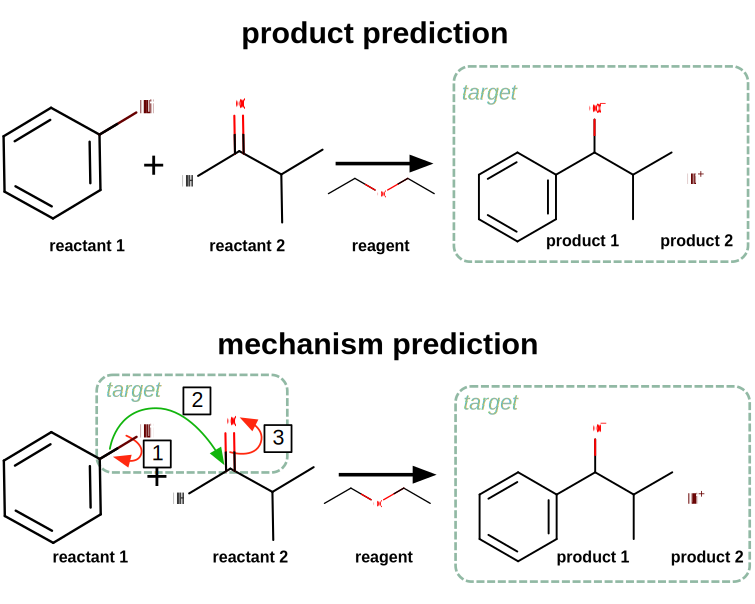
\includegraphics[width=\linewidth]{imgs/inkscape_img_edits/reaction_diagram.pdf}
    \col{.02}
    \col{.48}
      \begin{itemize}
        \item Reactions involve the stepwise movement of electrons along the atoms: this \colorize{breaks} and \colorize{forms} bonds.
        \item Recent approaches of ML applied to reaction prediction have focused on product prediction, we instead approach the problem from the angle
          of mechanism prediction: this provides \colorize{interprebility} and naturally \colorize{incorporates the constraints of chemistry} (eg balanced atom counts).
        \item We model reactions exhibiting linear electron flow (LEF) topology, the most common commong of reactions \citep{herges1994coarctate}.
      \end{itemize}
    \end{cols}


  }



  % \block{Commands}{
  %   \colorize{\bf Some nifty features:}
  %   Here are some of the commands we added to make life easier:
  %  \begin{enumerate} % verb// does not work inside of block
  %  \item {\tt fontscale} argument allows to scale all fonts (easy to refit poster)
  %  \item {\tt \textbackslash{}colorize\{test\}} makes text \colorize{colored} (automatically fitting to box color)
  %  \item {\tt \textbackslash{}s\{X\}} create a vertical space in units of em (relative to fontsize)
  %  \item {\tt cols} environment creating a multicolumn inside a box
  %    with {\tt \textbackslash{}col\{0.5\}} creating a new column with relative size
  %  \item {\tt \textbackslash{}ig[relsize]\{img\}} short for includegraphics with relative width to column (default 1.0)
  %  \end{enumerate}%

  %  \innerblock{interesting}{

  %    Normal text or \colorize{colorized text}
  %  }

  %  \s{1} % add some spacing
  %  \innerblock{}{
  %    box without header
  %  }

  %  \s{1}
  %  placing pics works great with cols environment (like in beamer with columns)
  %  \s{1}

  %  \begin{cols}
  %    \col{.4}
  %    \ig{logos/Max-Planck-Gesellschaft-black}
  %    \col{.2} \centering
  %    some text in between
  %    \col{.4}
  %    \ig{logos/Max-Planck-Gesellschaft-black}

  %  \end{cols}
  %}

  % COLUMN 2
  % ---------------------------------------------------------------------------
  \column{0.67}

  \block{Our model, \textsc{ELECTRO}, uses Graph Neural Networks to Parameterize the Probability of each kind of action}{

  }


\end{columns}

\block{We can extract these approximate electron paths from large scale reaction databases for training}{
blah}

\begin{columns}
  \column{0.4}

  \block{Assessing ability to predict paths}{
  blah2
}

  \column{0.4}

  \block{Assessing product prediction}{
  }

  \column{0.2}
%% References
  \block{}{
    % use bibtex here
    % \nocite*  % use this to force all entries in the bibfile to go here
    % \bibliography{mybib}
    % or the manual entries (can be copied from .bbl files in case you have used bibtex on a document)
    \setlength{\bibsep}{.5em}
    \begin{thebibliography}{1}

    \bibitem{Repo}
      Georg Martius and Dominik Zietlow.
      \newblock New MPI-IS poster style
      \newblock \url{https://gitlab.tuebingen.mpg.de/gmartius/posterstyle}, 2019

    \bibitem{tikzpackage}
      Richard Barnard, Elena Botoeva, Pascal Richter, and Dirk Surmann.
      \newblock tikzposter -- Create scientific posters using TikZ.
      \newblock \url{https://ctan.org/pkg/tikzposter}, 2014.

    \bibitem{herges1994coarctate}
     Rainer Herges.
     \newblock Coarctate transition states: The discovery of a reaction principle.
      \newblock Journal of chemical information and computer sciences, 1994.

    \end{thebibliography}
  }

\end{columns}

\end{document}
